\documentclass[doc,a4paper,12pt]{apa6}
\usepackage[utf8]{inputenc}
\usepackage[T1]{fontenc}
\usepackage[ngerman]{babel}
\usepackage{amsmath}
\usepackage[doublespacing]{setspace}
\usepackage{paralist}
\usepackage{graphicx}
\usepackage{epstopdf}
\usepackage{wrapfig}
\usepackage{float}
 
\title{Das Lernen einer komplexe Regelerkennung bei auditiven Stimuli}
\shorttitle{Explizite Komplexe Regelerkennung}
\author{Carlo Michaelis}
\date{23. August 2013}
\affiliation{Universität Leipzig}
\abstract{Abstract}
\ccoppy{Creative Commons (CC BY 3.0)}

\begin{document}

%\maketitle
%\newpage

%\tableofcontents
%\newpage

\section{Einleitung}

Viele Fragen sind bis heute ungeklärt und werden es wohl auch weiterhin bleiben. Trotzdem scheint es, als gäbe es – vor allem bei der Erklärung unserer physikalischen Umgebung – schon einige befriedigende Antworten, die nicht nur die notwendige Funktionalität ermöglichen, sondern Großteils bereits unseren Hunger nach Verständnis decken. In einem Bereich jedoch, dem Bereich psychischer Prozesse, gibt es zwar bereits viele Einzelerkenntnisse, eine umfassende Theorie über die psychischen Funktionsweisen komplexerer Organismen steht jedoch aus. Vor allem das Zusammenspiel, also die Schnittstelle zwischen der Psyche und dem Körper, die Frage nach Determiniertheit und Selbstbestimmung, nach Automatismus und Veränderbarkeit sind bei weitem noch nicht ganzheitlich geklärt.\\
Dabei erfüllt das Verständnis darüber nicht nur den Zweck Wissen über Lebewesen zu akkumulieren oder einige neugierige Personen zu befriedigen, vielmehr prägt die Erkenntnis über die Funktionsweise unsere Gesellschaft, sie entscheidet u.a. über Gesetze, Konventionen und Kultur.\\
So sehr wir uns als Menschen auch immer wieder selbstverständlich einen freien Willen unterstellen und damit die Fähigkeit durch den Geist gezielt und indeterminiert unsere Welt verändern zu können, ohne unwillkürliche Automatismen wäre ein Leben auf der Erde wohl unmöglich. In vielen Situationen müssen innerhalb kürzester Zeit bestehende Reize erfasst, zukünftige Ereignisse simuliert und schließlich vorhergesagt werden.

Ein gutes Beispiel für die hohe Leistungsfähigkeit der automatisch ablaufenden Systeme des Menschen ist seine Sprache. Deutlich wird dies schon allein durch das Segmentationsproblem beim Sprachverstehen. Mit physikalischen Mitteln aufgezeichnete Frequenzen von Schallwellen zeigen Muster, die bei visueller Betrachtung kaum korrekt in Worte getrennt werden können. Eine Pause oder eine Frequenzschwankung sagt nur selten tatsächlich auch den Beginn eines neuen Wortes vorher. Zur Segmentation der Worte werden bei weitem nicht nur die physikalischen Signale, sondern zusätzlich viele verschiedene Hinweisreize benötigt (u.a. Saffran, Newport \& Aslin, 1996; Brent \& Cartwright, 1996). Die Segmentation muss jedoch nicht nur anhand einer großen Menge an Informationen, sondern auch innerhalb kürzester Zeit erfolgen, die ohne eine automatisierte Vorhersage wohl kaum möglich wäre.\\
Beim Sprechen wiederum ist zum Beispiel das so genannte Speech Monitoring (Levelt, 1983; Postma, 2000) von hoher Bedeutung. Das bezeichnet die Fähigkeit die inhaltliche Qualität des gesprochenen noch während dem Sprechen reflektieren zu können. Das bedeutet wiederum, dass beim Sprechen mindestens zwei Prozesse gleichzeitig ablaufen. Das legt nah, dass hier ein hoher Automatismus-Grad im Spiel ist. In einer Studie von Goldmann-Eisler (1958) konnte gezeigt werden, dass u.a. immer dann größere Sprechpausen entstehen, wenn kommende Wörter schwerer vorhersagbar sind. Umgekehrt scheint Sprache also auch entscheidend von der Fähigkeit zur Vorhersage abhängig zu sein.\\
Bezüglich der auditiven Komponente sei vor allem auch die Musik hervorgehoben. Gerade in der Musik spiegelt sich die Tendenz des Menschen zu erfolgreichen Vorhersagen wieder. Drake und Bertrand (2001) prüften 5 universelle, d.h. nicht-kulturabhängige Paradigmen, wie sich Menschen zu Musik verhalten. In Paradigma 3 beschrieben sie, dass sich Menschen, die im Takt der Musik bleiben sollen, in mehr als 90\% der Zeit erfolgreich mit Musik synchronisieren können. D.h. sie können Vorhersagen erfolgreich treffen und ihre Handlung auch entsprechend erfolgreich an den Vorhersagen steuern. Man könnte mutmaßen, dass genau in der Vorhersagbarkeit der Reiz der Musik liegt und auch ein Harmonieempfinden damit zusammenhängt.

Die Bedeutung der Vorhersagbarkeit und vor allem der diesbezüglich wirkenden Automatismen lässt sich an den vorigen Beispielen recht gut erkennen. Im folgenden Experiment soll es um die Vorhersagbarkeit von komplexen Regeln in auditiven Stimuli gehen. Konkret soll untersucht werden inwiefern komplexe Regeln von Tonabfolgen (wie sie etwa auch in der Sprache vorkommen) erkannt und insbesondere vorhergesagt bzw. Abweichungen erkannt werden können. Im Folgenden soll zunächst der Forschungsstand bezüglich der auditiven Regelerkennung erläutert werden. Anschließend wird eine kurze Einführung in Lerntheorien erfolgen, die speziell für dieses Experiment von Bedeutung sein wird.

\subsection{Missmatch Negativity (MMN) und das Oddball Paradigma}

Die Missmatch Negativity (MMN) ist ein ereigniskorreliertes Potential (EKP). Bei ereigniskorrelierten Potentialen handelt es sich um elektrische Potentiale des Gehirns, welche zu einem bestimmten Zeitpunkt (Ereignis) eintreten und mit diesem Zusammenhängen und daher als ereigniskorreliert betrachtet werden können. Die Messung dieser Signale erfolgt per Elektroenzephalogramm (EEG), welches elektrische Potentiale des Gehirns erfassen kann. Um die Signale des Ereignisses letztlich vom Rauschen anderer Gehirnpotentiale trennen zu können, werden die Potentiale über mehrere Messungen gemittelt.

Erstmals wurde die MMN von Näätänen, Gaillard \& Mäntysalo (1978) für auditive Stimuli beschrieben. Verwendet wurde das so genannte Oddball Paradigma, bei dem eine Reihe gleicher Stimuli gegeben wird, welche dann von einem nicht-regelkonformen Stimulus unterbrochen wird. Die MMN trifft dann ca. 150ms – 250ms nach der Präsentation des Abweichers vor allem im fronto-zentralen Bereich auf. Sie zeigt damit an, dass eine Vorhersage (bzw. eine Extrapolation) des Gehirns fehlerhaft ist. Im Umkehrschluss lässt sich bei einem Auftreten der MMN schließen, dass das Gehirn zuvor eine Regelmäßigkeit erkannt haben muss. Diese Ableitung wurde auch in den Studien verwendet, die diesem Experiment zugrunde liegt.

Eine weitere Eigenschaft der MMN ist, dass sie auch dann auftritt, wenn der auditive Stimulus nicht beachtet wird. Z.B. wenn Probanden während dem Hören der Töne einen Stummfilm schauen.\\
Das Gehirn scheint also keine (oder nur sehr wenige) Aufmerksamkeitsressourcen für die Erkennung einer Regelmäßigkeit in einem auditiven Stimulus zu benötigen und die Verarbeitung erfolgt damit relativ automatisch.

\subsection{Komplexe Regelerkennung}

Es stellte sich schon bald die Frage, ob die MMN auch bei deutlich komplexeren Regeln auftritt. Dies würde – oben bereits genannt – implizieren, dass das Gehirn die Fähigkeit besitzt komplexe Regeln zu extrahieren und vorhersagen zu können.\\
Die ersten Paradigmen zur Untersuchung komplexerer Regeln bei auditiven Stimuli ergaben, dass die Regeln zwar vom Gehirn erkannt (gemessen per MMN), jedoch nicht bewusst verarbeitet werden konnten. Im Sequence Learning Paradigm (Hoffmann \& Koch, 1998) sollten die Probanden ein sich wiederholendes Muster erkennen, welches in einer Ton-Sequenz versteckt war, im Covariation Detection Paradigm (Stamov Rossnagel 2001) wiederum lernten die Probanden nichtsaliente Verbindungen zwischen den einzelnen Stimulus-Elementen. Obwohl die Probanden die Regeln meist nicht bewusst erkannten, zeigten sich durch Übung Leistungssteigerungen in Form von zunehmend erhöhter Geschwindigkeit und erhöhter Genauigkeit, was zunächst auf implizites Lernen hinweist.

Paavilainen, Arajärvi \& Takegata (2006) warfen daraufhin die Frage auf in welchem Ausmaß der Erkennungsprozess Aufmerksamkeitsressourcen benötigt. Dabei sollte vor allem geklärt werden, ob die Regelerkennung komplexerer Regeln eventuell bereits präattentiv auf der Ebene des sensorischen Gedächtnisses stattfindet. Um dies zu untersuchen wurden den Probanden je 2000 Töne vorgespielt, die sich in ihrer Länge (50ms oder 150ms) und in ihrer Höhe (1000Hz oder 1500Hz) unterschieden. Dabei konnten zwei gegensätzliche Regeln vorkommen:

\begin{compactitem}
  \item Auf einen langen Ton folgt ein hoher Ton, auf einen kurzen Ton folgt ein tiefer
Ton
  \item Auf einen langen Ton folgt ein tiefer Ton, auf einen kurzen Ton folgt ein hoher
Ton
\end{compactitem}

Von den zwei Merkmalen (Höhe und Länge) ist jeweils die Länge der entscheidende Prädiktor für das Merkmal Höhe des nächsten Tons. Eine Beispielsequenz dieser Regel ist in Abbildung 2 im Abschnitt Methoden zu sehen.\\
Alle Probanden durchliefen in gegebener Reihenfolge folgende Bedingungen:

\begin{compactitem}
  \item \textbf{Ignore}: Die Probanden schauten einen Stummfilm mit Untertiteln und sollten nicht auf die Töne reagieren.
  \item \textbf{Implicit detection}: Den Probanden wurde die Regel nicht erklärt, sie sollten jedoch eine Taste drücken wenn sie das Gefühl hätten, dass ein Ton nicht passt.
  \item \textbf{Explicit detection}: Den Probanden wurde die Regel erklärt (mit Hilfe eines Schaubildes), sie sollten eine Taste drücken, wenn der letzte Ton von der Regel abweicht.
\end{compactitem}

Im Ergebnis zeigte sich, dass in allen drei Bedingungen der Ausschlag der MMN nicht signifikant voneinander abweicht. Es war also unerheblich, ob die Probanden den Ton ignorierten oder aktiv darauf achteten. Auch implizite, so wie explizite Lernprozesse waren demnach anscheinend nicht vorhanden. Für einen - zumindest kleinen - Lerneffekt spricht hingegen, dass die behavioralen Daten in den zwei detection-Bedingunen in Form der Erfolgsrate beim Drücken der Tasten signifikant vom Zufall abwichen, wenn auch nur sehr gering. Qualitativ wurde außerdem berichtet, dass die Probanden das Wissen über die Regel nur als wenig hilfreich einschätzten.\\
Aus den Ergebnissen wurde geschlossen, dass die Verarbeitung wohl überwiegend automatisiert und die Treffer in der explicit detection Bedingung eher auf Intuition, als auf explizites Wissen über die Regel zurückzuführen ist. Allerdings scheinen die neuronalen Mechanismen, die auch die MMN auslösen ihre Leistungsfähigkeit verbessern zu können. Dies schlägt sich zumindest in der knapp überzufälligen Erfolgsrate nieder. Letztlich war ein weiteres EKP, die so genannte P300, nicht ausgeprägt. Diese Komponente schlägt üblicherweise aus, wenn Stimuli bewusst klassifiziert werden. Die These, dass die Stimuli automatisiert und unbewusst verarbeitet werden konnte auch damit bestätigt werden.

Die Studie von Paavilainen, Arajärvi \& Takegata (2006) wurde 2 Jahre später von Bendixen, Prinz, Horváth, Trukillo-Barreto \& Schröger (2008) repliziert und erweitert. Dabei wurden die gleichen Regeln verwendet, auch Tonhöhe und Frequenz entsprach den vorigen.\\
Die Regeln wurden in unterschiedlich langen Sequenzen (4, 9, 14, 19 Töne) regelkonform präsentiert und anschließend durch irreguläre Sequenzen (4-8 Töne) unterbrochen. Diese Unterbrechung führt dazu, dass das Gehirn immer wieder von vorne beginnen muss eine Regel zu erkennen, zumal nach einer irregulären Sequenz auch die reguläre Sequenz variieren kann, da wie oben beschrieben, zwei solcher regulären Regeln existieren. Es wurde zwischen zwei Bedingungen unterschieden:

\begin{compactitem}
  \item \textbf{Passiv}: Kontinuierliche Stimuli-Präsentation, wobei dir Probanden einen Stummfilm schauten und Stimuli ignorieren sollten.
  \item \textbf{Aktiv}: Probanden hörten abgegrenzte Sequenzen (6, 11, 16, 21 Töne), wobei letzter Ton Standard oder Deviant sein sollte. Sie bekamen die Regeln erklärt und sollten per Tastendruck reagieren.
\end{compactitem}

Die Probanden bekamen erst 8 Blöcke in der Passiv-Bedingung präsentiert, wurden gefragt, ob sie eine Regel erkannten, anschließend bekamen sie 5 weitere Blöcke in der Aktiv-Bedingung präsentiert. In keinem Fall erkannten die Probanden die Regel nach der Passiv-Bedingung korrekt, sofern sie überhaupt eine erkannten. Die Sensitivität (d-prime) lag noch signifikant über dem Zufallsniveau, sowohl für kurze (5 und 10 Töne), als auch für lange (15 und 20 Töne) Sequenzen. Die MMN zeigte jedoch nur für lange Sequenzen eine signifikante Ausprägung.\\
Die Ergebnisse von Paavilainen et al. konnten damit zum einen bestätigt werden, zum anderen konnte gezeigt werden, dass für die Regelerkennung zunächst einige Stimuli nötig sind, bis das Gehirn die entsprechende Regel abgeleitet hat. Allgemein liegt ein kontinuierlicher Zusammenhang vor. Je mehr regelkonforme Stimuli präsentiert werden, desto höher ist der Ausschlag der MMN. Es scheint also eine Akkumulation von Hinweisen auf eine Regel vorzuliegen. Entscheidend ist jedoch, dass auch in dieser Studie das bewusste Erkennen einer Regelverletzung nicht möglich war. Auch hier zeigte sich die Abwesenheit der P300-Komponente und damit die Abwesenheit bewusster Klassifikationsprozesse.

% ##################################################
% P300? In der Studie ist sie als P3a bezeichnet. Wenn ich es richtig verstanden habe, dann wird die P300 eigentlich als P3b bezeichnet. Nun war ich ein wenig verwirrt und habe es der Einheitlichkeit halber einfach auch P300 genannt
% ##################################################

\subsection{Lernen prozeduralen Wissens}

Zusammenfassend liegt also bezüglich der Erkennung komplexer Regeln eine automatisierte und unbewusste Verarbeitung vor. Für eine weitere Untersuchung ist es zunächst von Bedeutung zu betrachten wie das implizite und explizite prozedurale Lernen funktioniert. Daraus könnte abgeleitet werden wie ein expliziter prozeduraler Lernprozess komplexer Regeln gestaltet werden könnte. Sollte dieser erfolgreich sein könnte dies ein Ansatz sein um die Funktionsmechanismen hinter der Lücke zwischen der automatisierten unbewussten und der manuellen bewussten Verarbeitung zu verstehen.

Grundsätzlich lässt sich der Lernprozess recht eindeutig als prozedurales Lernen (abgegrenzt von deklarativem Lernen) klassifizieren, sofern das Drücken der Taste passend zu den Abweichlern gelernt wird. Außerdem lag in den bisherigen Untersuchungen – wenn überhaupt – nur implizites Lernen vor. Interessant wäre also zu betrachten wie explizites Lernen erreicht werden kann, welches bisher den Probanden nicht möglich war. Prinzipiell ist auf Grund der genannten Ergebnisse vermutlich davon auszugehen, dass sich ein expliziter Lernprozess relativ schwierig gestalten könnte.

Die Klassifikation in prozedurale Prozesse macht nun deutlich, dass ein einfaches Zeigen der Regel (z.B. an einem Schaubild) kaum ausreichen kann, um die Regel adäquat anzuwenden. Zumal die Stimuli mit 50ms bzw. 150ms Länge und einem Inter-Stimulus-Intervall (ISI) von 300ms präsentiert wurden. Diese hohe Geschwindigkeit erfordert wahrscheinlich ein langes Training, sofern ein expliziter Prozess verlangt wird.

Fitts und Posner (1967) gingen davon aus, dass prozedurales Wissen über drei Schritte hintereinander gelernt werden kann:

\begin{compactenum}
  \item \textbf{Kognitives Stadium}: In diesem Stadium handelt es sich noch um eine deklarative Repräsentation. Das deklarative Wissen kann in bestehendes Wissen integriert und mit diesem verknüpft werden. Eine Vermittlung sollte präzise und verständlich erfolgen. Angewendet werden kann z.B. ein Schaubild.
  \item \textbf{Assoziatives Stadium}: Eine prozedurale Repräsentation wird aufgebaut. Es entwickeln sich Wenn-Dann-Regeln. Sofern ein bestimmtes Ereignis eintritt wird automatisch eine spezifische Reaktion ausgeführt. Dieses Stadium kann vor allem durch regelmäßige Übung erreicht werden. Wichtig ist hier auch das Geben von Feedback.
  \item \textbf{Autonomes Stadium}: Das prozedurale Wissen kann schnell und automatisiert abgerufen werden. Die einzelnen Repräsentationen sind stabil miteinander verbunden und führen zu einer fehlerfreien Ausführung. Der Ressourcenaufwand minimiert sich. Erreicht wird dies durch das Praktizieren über längere Zeiträume.
\end{compactenum}

Eine gute Beschreibung des prozeduralen Lernens bietet auch der Learning Cycle von Withmore (2009). Der Kreislauf teilt das Lernen in 4 aufeinanderfolgende Schritte ein:

\begin{compactenum}
  \item \textbf{Unconscious incompetence}: Kein Verständnis vorhanden
  \item \textbf{Conscious incompetence}: Es liegt zwar nur eine geringe Performanz vor, Fehler und Schwächen werden jedoch bemerkt und können korrigiert werden
  \item \textbf{Conscious competence}: Die Leistung verbessert sich, zur Durchführung ist jedoch ein hoher kognitiver Aufwand nötig
  \item \textbf{Unconscious competence}: Es liegt eine hohe Performanz vor, der kognitive Aufwand verringert sich deutlich zugunsten automatisierter Abläufe
\end{compactenum}

Warum ein explizites Lernen in den vorigen Studien wahrscheinlich nicht möglich war kann nun auf Basis der beiden Modelle sehr schnell erklärt werden. Unter der Voraussetzung, dass prozedurales Wissen vorliegt und gelernt werden muss wurde in beiden Studien vermutlich lediglich das kognitive Stadium erreicht (nach Fitts \& Posner, 1967). Es wurden zwar Übungsdurchgänge vorgenommen, diese waren aber direkt in der Standard-Geschwindigkeit. Die Wahrscheinlichkeit, dass stabile Wenn-Dann-Regeln aufgebaut werden konnten ist sehr gering, da die Versuchspersonen vermutlich auf Grund der Überforderung keine Möglichkeit hat ihr Verhalten adäquat zu überdenken (fehlendes Feedback) und der Schwierigkeitsgrad zu abrupt ansteigt. Nach der Annahme der Zone proximaler Entwicklung von Wygotski (Kozulin, 2003) sollte der nächste Lernschritt knapp über dem aktuellen Lernniveau sein, um ein optimales Lernen zu gewährleisten. Diese Bedingung war bisher nicht gegeben.\\
Nach dem Modell von Withmore dürften die Probanden sogar nicht einmal über die erste Stufe hinaus gekommen sein, da Fehler und Schwächen nicht bemerkt werden. Es dürfte demnach also keine Verbesserung der Leistung eintreten können.

\subsection{Hypothese}

Es soll an dieser Stelle zunächst noch einmal der aktuelle Stand aus den bisher genannten Informationen zusammengefasst werden:

\begin{compactitem}
\item Der Mensch (und vermutlich auch andere höhere Organismen) besitzen die Fähigkeit hochautomatsiert und daher mit hoher Geschwindigkeit und Präzision Regeln zu erkennen.
\item Das Erkennen der Regeln führt zu der Fähigkeit zukünftige Ereignisse vorhersagen zu können.
\item Diese Fähigkeit funktioniert insbesondere auch für komplexe Regeln und ohne bewusste Aufmerksamkeit.
\item Der bewusste Zugriff und das bewusste Lernen dieser Regeln ist sehr schwer.
\item Die manuelle bewusste und die automatisierte unbewusste Verarbeitung basiert vermutlichen auf unterschiedlichen Verarbeitungsprozessen. Die automatisierte Verarbeitung wird bereits auf sensorischer Ebene vermutet.
\end{compactitem}

Die bisherigen Ergebnisse werfen einige Fragen auf, welche Schrittweise verstanden werden wollen, um den Unterschiede zwischen den Verarbeitungsmechanismen verstehen zu können. Ein erster Schritt wurde in diesem Experiment getestet. Dabei wurde die Frage gestellt ob und wenn ja unter welchen Umständen ein explizites Lernen möglich ist. Dafür wurde folgende Hypothese formuliert:

\textbf{Hypothese}: Das Lernen der komplexen Regeln sollte unter Beachtung der Lerntheorien für prozedurales Wissen auch explizit möglich sein.

Während bisher bisher die Regel einfach erklärt wurde, soll im folgenden ein theoretisch abgeleitetes Lernkonzept angewendet werden. Dabei wird der Schwerpunkt auf der 3-stufigen Theorie von Fitts und Posner (1967) liegen. Beachtet werden soll außerdem die Zone proximaler Entwicklung. Im folgenden Methoden-Teil wird die Hypothese unter Beachtung der Experimentalbedingungen noch einmal präzisiert.


\section{Methoden}

\subsection{Probanden}

Insgesamt wurden für die Untersuchung 21 Probanden getestet. Zwei entfielen auf die Pilotierung, eine weitere Person musste wegen technischen Problemen während des Versuchsdurchgangs aus den Daten genommen werden. Von den verbleibenden 18 Probanden waren 3 männlich (16.7\%) und 15 weiblich (83.3\%). Das Durchschnittsalter betrug 27 Jahre (SD = 8), die Probanden variierten zwischen einem Alter von 18 und 53 Jahren. Von den 18 Probanden fühlten sich 11 gut ausgeschlafen und 13 gut konzentriert. Die übrigen hatten mindestens mäßig geschlafen und waren mindestens mäßig Konzentriert, entsprechend hatte kein Proband schlecht geschlafen oder war schlecht konzentriert. Keiner der Probanden nahm im Voraus Substanzen zu sich, die das Nervensystem hätten beeinträchtigen können und alle Probanden konnten gut hören und den Experimentalbedingungen entsprechend ausreichend sehen. Eine Versuchsperson musste in Englisch instruiert werden, die Aufgabe wurde jedoch ohne Schwierigkeiten verstanden.

\subsection{Versuchsaufbau}

In Abbildung 1 ist eine Skizze des Versuchsaufbaus gezeigt. Das Experiment musste unter nicht ganz optimalen Experimentalbedingungen durchgeführt werden, da sich die Labore der Professur für Kognitive einschließlich Biologische Psychologie zum Erhebungszeitpunkt gerade im Umbau befanden. Um trotzdem möglichst optimale Bedingungen zu erhalten wurde versucht eine Reihe von Maßnahmen zu treffen.

\newpage

\begin{wrapfigure}{r}{.6\textwidth}
  \centering
  \begin{minipage}{.55\textwidth}
    \setlength{\fboxsep}{.05\textwidth}
    \fbox{\begin{minipage}{.95\textwidth}
      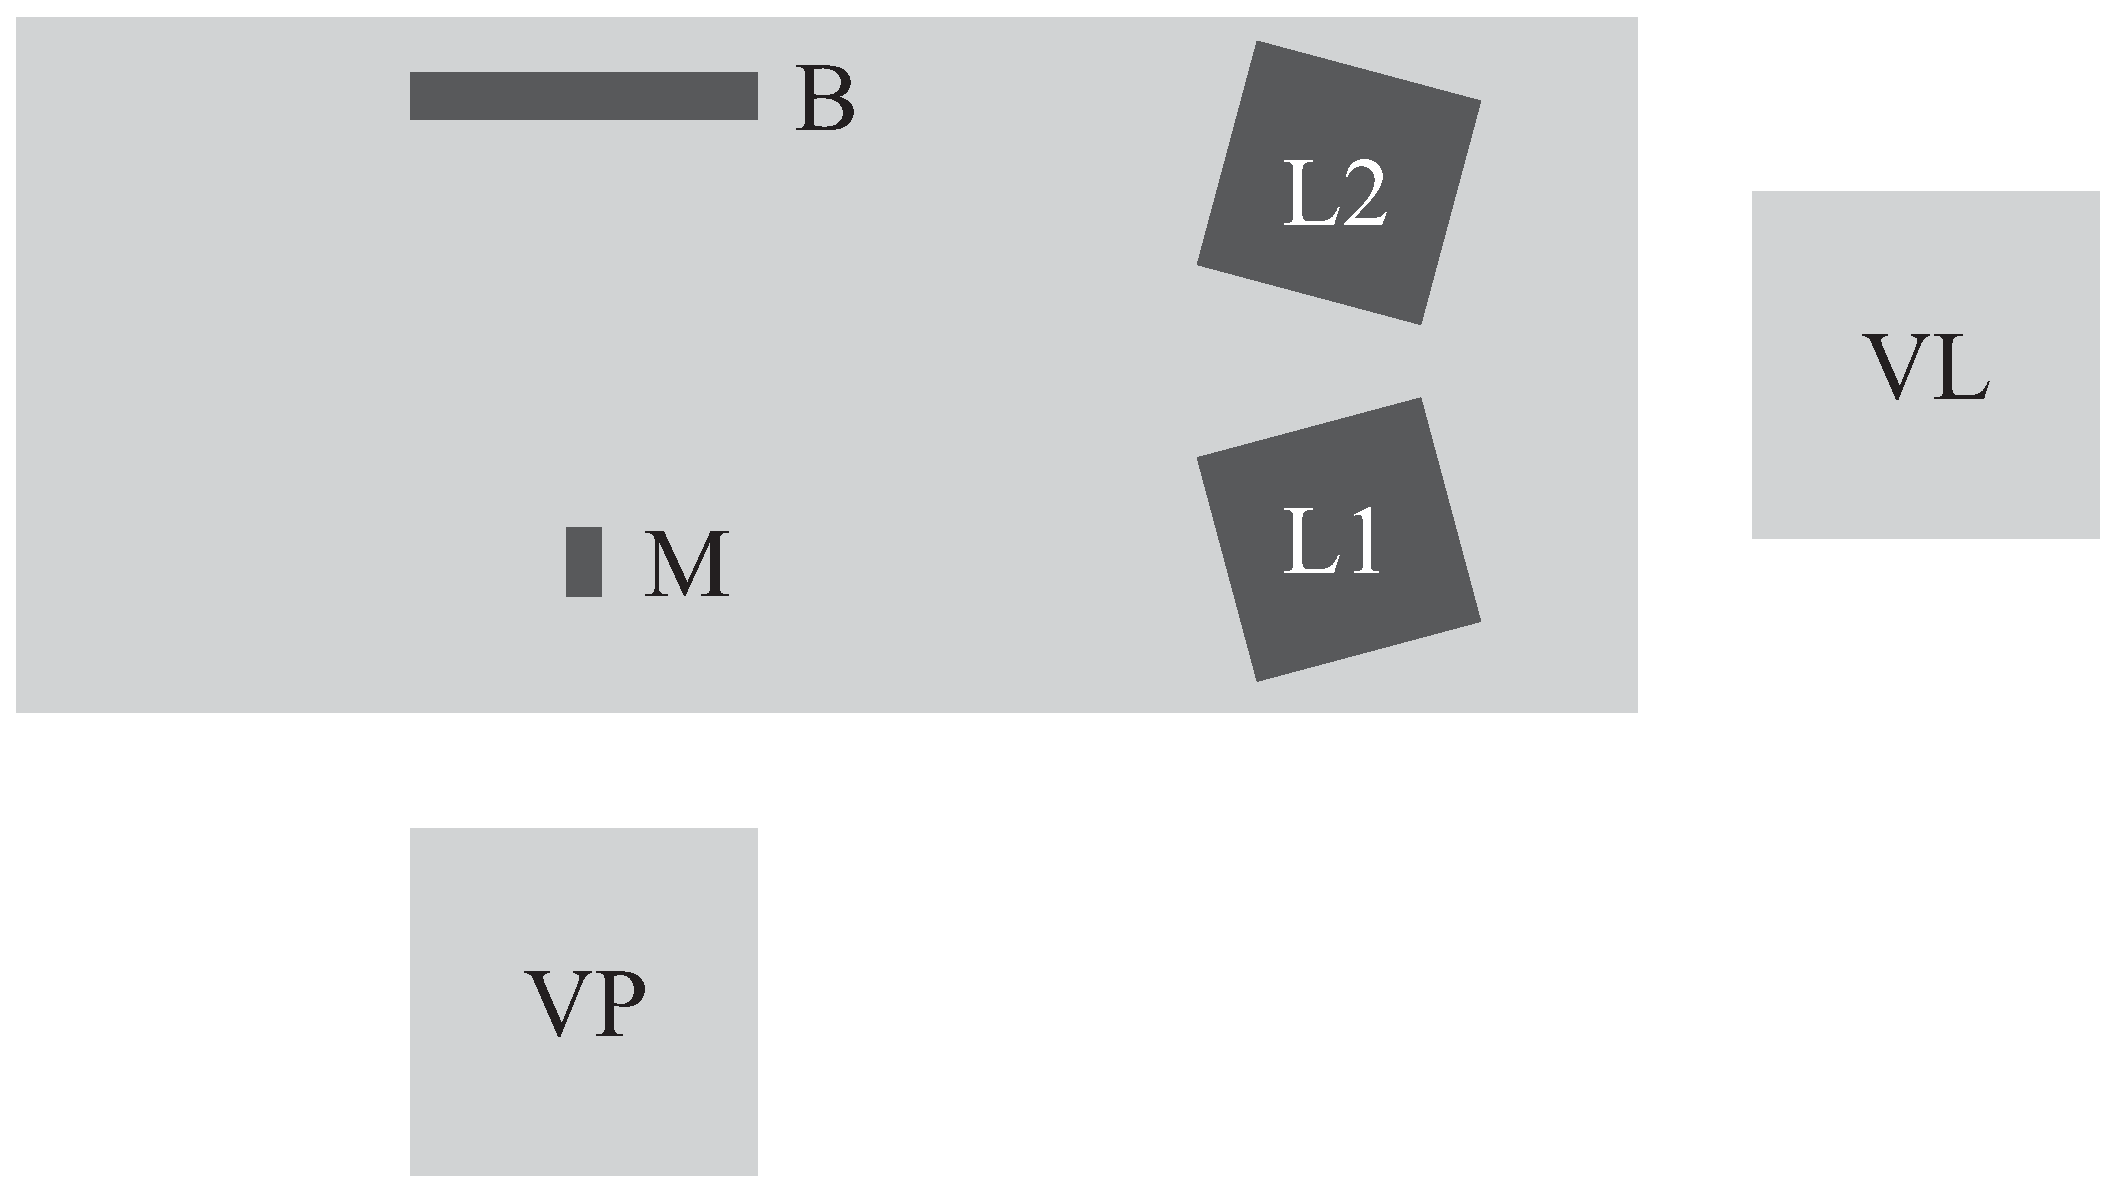
\includegraphics[width=\textwidth]{abb1-versuchsaufbau.eps}
    \end{minipage}}
    \vspace{10pt}
    \caption{Aufbau des Experimentes. Laptop 1 (L1) mit Programm für Experiment und Laptop 2 (L2) für Experimentator (E). Bildschirm (B), Maus (M) und Kopfhörer (nicht eingezeichnet) für Versuchsperson (VP).}
  \end{minipage}
  \vspace{-15pt}
% ################
% Anhang ergänzen!
% ################
\end{wrapfigure}

% ################
% Caption korrekt?
% ################

Auf Laptop 1 (L1) wurde das Programm für den Versuch ausgeführt, dieser wurde vom Experimentator (E) bedient. Dieser Laptop war an den Bildschirm (B) angeschlossen, welcher der Versuchsperson (VP) zur Verfügung stand. Auf diesem Bildschirm wurde angezeigt, wenn die Versuchsperson reagieren sollte. Zur Reaktion stand der Versuchsperson eine Computer-Maus (M) mit 2 Tasten zur Verfügung. Des Weiteren wurde ein zweiter Laptop (L2) verwendet. Dieser wurde verwendet, damit sich Experimentator (E) während den Blöcken ablenken konnte. Unter Experimentalbedingungen im Labor sind Experimentator und Versuchsperson räumlich getrennt. In diesem Fall war eine räumliche Trennung nicht möglich. Um etwaige Versuchsleitereffekte zu minimieren, sollte der Experimentator nicht den Eindruck vermitteln die Versuchsperson zu beobachten oder gar zu kontrollieren. Auch subtile Reaktionen des Experimentators auf eventuelles gutes oder schlechtes Abschneiden der Versuchsperson sollten vermieden werden, indem der Experimentator von vorne herein den Bildschirm von L1 maximal abdunkelte und diesen nach Möglichkeit nicht beachtete. Die Ablenkung an L2 erfolgte durch kognitiv anstrengende Aufgaben. Dabei wurde beachtet, dass der Experimentator nach dem Ende eines Blockes unverzüglich wieder zur Versuchsperson umschalten musste. Die Versuchsperson musste nach Beendigung eines Blockes ohne Unterbrechung direkt die volle Aufmerksamkeit bekommen, um die Motivation aufrecht zu erhalten und keinen Eindruck von Desinteresse zu vermitteln.

Um Störungen von außen zu vermeiden wurde ein Schild an die Tür angebracht, welches darauf hinwiese, dass in diesem Raum ein Experiment am Laufen ist. Außerdem wurde das Fenster geschlossen und die Kopfhörer wurden vorher auf eine normierte Lautstärke eingestellt. Alle Utensilien (Maus, Kopfhörer, Formulare) wurden vorpräpariert auf den Tisch gelegt (bei Position M). Auch alle Einstellungen am Programm wurden vor der Ankunft der Versuchsperson vorbereitet, der Bildschirm (B) war zunächst ausgeschaltet und wurde erst unmittelbar vor dem Start des Versuchs eingeschaltet.

\subsection{Stimuli}

Innerhalb der Blöcke bekam die Versuchsperson auditive Stimuli präsentiert. Diese bestanden aus Tonsequenzen à 10, 15 oder 20 Tönen. Dabei waren die Töne und die Regel entsprechend denen bei von Paavilainen et al. (2006). Die Töne unterschieden sich in Länge (hoch/tief) und Länge (kurz/lang). Dabei wurden die Frequenzen für hohe (1500Hz) und tiefe (1000Hz) Töne wie zuvor verwendet. Auch die Länge der Töne blieb mit 50ms für Kurze und 150ms für lange Töne identisch den vorigen Experimenten. Die Regel für die Töne lautete wie zuvor bereits in der Einleitung beschrieben:

\begin{compactitem}
  \item Auf einen langen Ton folgt ein hoher Ton, auf einen kurzen Ton folgt ein tiefer
Ton
  \item Auf einen langen Ton folgt ein tiefer Ton, auf einen kurzen Ton folgt ein hoher
Ton
\end{compactitem}

\newpage

\begin{figure}
  %\vspace{10pt}
  \centering
  \begin{minipage}{\textwidth}
    \setlength{\fboxsep}{.05\textwidth}
    \fbox{\begin{minipage}{.9\textwidth}
      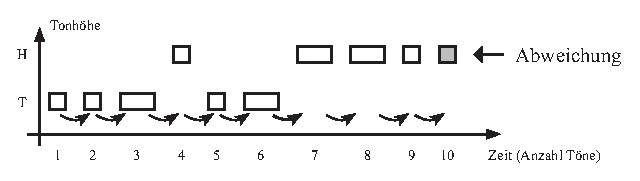
\includegraphics[width=\textwidth]{abb2-tones.eps}
    \end{minipage}}
    \vspace{10pt}
    \caption{Beispiel für eine Tonsequenz. Die Länge des einen Tons sagt die Höhe des nächsten Tons vorher. In diesem Beispiel folgt auf einen kurzen Ton ein tiefer Ton und auf einen langen Ton ein Hoher Ton. Der letzte Ton ist im Beispiel von der Regel abweichend. Auf einen kurzen Ton (Ton 9) folgt kein tiefer Ton, wie die Regel es vorhersagen würde, sondern ein hoher Ton (Ton10).}
  \end{minipage}
  \vspace{-5pt}
\end{figure}

Unterschiede gab es zum einen beim Inter-Stimulus-Intervall (ISI), welches zwischen den Blöcken variierte. Angewendet wurden Intervalle von 300ms, 600ms und 900ms. Zum anderen bildete der letzte Ton in 50\% der Fälle eine Ausnahme und wich von der gegeben Regel ab. Dabei wurden die Sequenzen nicht kontinuierlich präsentiert. Die nächste Sequenz startete erst, sobald ein Tastendruck ausgeführt wurde. In Abbildung 2 ist eine Beispielsequenz mit einer Abweichung am Ende skizziert.\\
Die Versuchsperson sollte mit der Maus nun darauf reagieren und entscheiden, ob der der letzte Ton passend oder abweichend ist. Dem zufolge liegt die Leistung der Versuchsperson darin zunächst die Regel zu erkennen, die letzten, zuletzt gespielten Töne im Gedächtnis zu behalten und nach Beendigung eine Entscheidung zu treffen. Auf dem Bildschirm war während den Sequenzen ein Fixationskreuz zu sehen, welches unmittelbar nach dem letzten Ton der Sequenz in ein Fragezeichen wechselte. Da die Sequenzen unterschiedlich lang waren, sollte dieses Hilfsmittel die Unsicherheitszeit zwischen den Sequenzen, die mindestens dem Inter-Stimulus-Intervall entspricht, möglichst gering zu halten. Eine Reaktionszeit-Variation zwischen den Blöcken sollte damit vermieden werden.

\subsection{Ablauf}

Der Ablauf des Experimentes erfolgte nach einer standardisierten Checkliste. Damit konnte der Experimentator überprüfen, ob nach jedem Schritt alle relevanten Punkte erläutert wurden. Die Liste war für die Versuchsperson nicht sichtbar. Folgender Ablauf wurde durchgeführt:

\begin{compactenum}
  \item \textbf{Vorbereitung}: Präparation des Versuchsraumes (vor dem Eintreffen der VP)
  \item \textbf{Einführung}: Erklärung des Experimentes
  \item \textbf{Block 1 (schnell)}: Durchgang mit ISI von 300ms
  \item \textbf{Arbeitsblatt}: Lernen der Regel mit Hilfe eines Arbeitsblattes
  \item \textbf{Block 2 (langsam)}: Durchgang mit ISI von 900ms und Feedback
  \item \textbf{Block 3 (mittel)}: Durchgang mit ISI von 600ms und Feedback
  \item \textbf{Block 4 (schnell)}: Durchgang mit ISI von 300ms
  \item \textbf{Nachbereitung}: Präparation des Versuchsraumes (vor dem Eintreffen der VP)
\end{compactenum}

Die Variation der ISI zwischen den Blöcken ist, ebenso wie das Arbeitsblatt, ein Lernprozess im Sinne der Lerntheorie von Fitts und Posner (1967). Dabei repräsentiert das Arbeitsblatt das kognitive Stadium mit einem Übergang in das assoziative Stadium. Block 2 und Block 3 bilden das assoziative Stadium und sollten im Idealfall in Block 4 in das autonome Stadium überführen.

\subsubsection{(1) Vorbereitung}

In der Vorbereitung wurde das Mobiltelefon auf Stumm geschaltet, die Lautstärke (Windows 7 Betriebssystem) auf 40 eingestellt und der Laptop-Bildschirm abdunkelt. Außerdem wurde das Fenster geschlossen (sofern vorher gelüftet wurde), Formulare und Stift, sowie Kopfhörer und Maus wurden bereitgelegt. Letztlich wurden einige Minuten für einen Moment der Ruhe eingeplant um konzentriert, klar und ruhig mit der folgenden Versuchsperson umgehen zu können.

\subsubsection{(2) Einführung}

Nach dem Unterschreiben der Formulare wurden die Rahmenbedingungen des Experimentes erklärt. Dabei wurde beim ersten Durchgang noch nicht die Regel erklärt. Der erste Durchgang dient als Kontrolldurchgang. Der Versuchsperson wurden folgende Fakten erklärt:

\begin{compactitem}
\item Eine Sequenz besteht aus 10-20 Tönen
\item Ein Block besteht aus 24 Sequenzen
\item Die Töne unterscheiden sich in Höhe (hoch/tief) und Länge (kurz/lang)
\item Der letzte Ton einer Sequenz kann zu den vorigen passen oder nicht passen
\item Eine Maustaste für "passt", eine für "passt nicht"
\item Erster Durchgang intuitiv
\end{compactitem}

Ergänzt wurde außerdem, dass der Experimentator während den Blöcken keine Ergebnisse beobachtet und sich an Laptop 2 ablenken wird. Außerdem wurde der Versuchsperson verdeutlicht, dass Genauigkeit wichtig ist. Letztlich bekam die Versuchsperson noch eine Empfehlung zur Bedienung der Maus. Die Tastenbelegung der Maus variierte zwischen den Versuchspersonen gleichmäßig, um eventuelle Effekte von Händigkeit auszuschließen. Die Versuchsperson bekam die Tastenbelegung vor jedem Block auf einem Startbildschirm angezeigt.

\subsubsection{(3) Block 1}

In Block 1 wurde zunächst ein Inter-Stimulus-Intervall von 300ms verwendet. Dies entspricht dem ISI von Paavilainen et al. (2006) und Bendixen et al. (2008). Nach dem der erste Block beendet war, wurde die Versuchsperson gefragt, ob sie eine Regel erkannt hatte. Sofern die Versuchsperson dies verneinte oder keine korrekte Regel nannte, wurde die Versuchsperson durch den Experimentator ermutigt mit der Aussage, dass noch niemand jemals zu diesem Zeitpunkt eine Regel erkannt habe und das Nicht-Erkennen der Regel ein wichtiger Bestandteil des Experimentes ist.

\subsubsection{(4) Arbeitsblatt}

In diesem Schritt, unmittelbar nach Block 1, wurde der Versuchsperson ein Arbeitsblatt (siehe Anhang) gegeben. Dafür setze sich der Experimentator neben die Versuchsperson an die lange Kante des Tisches neben Position VP. Das Arbeitsblatt wurde in allen Fällen gemeinsam bearbeitet. Dabei wurde zunächst anschaulich die Regel erklärt. Anschließend war die Versuchsperson aufgefordert für beide Regeln je eine eigene Sequenz zu erfinden und zu zeichnen. Bis zu diesem Punkt handelte es sich noch um die kognitive Stufe. Auf der letzten Seite des Arbeitsblattes wurde dann in die assoziative Stufe gewechselt. Dort waren Sequenzen vorgegeben, bei denen bestimmt werden musste, ob der letzte Ton regelkonform oder abweichend ist. Diese Übung entsprach in visuell/bildlicher Form der auditiven Übung und sollten der Festigung der verstandenen Regel dienen. Nach Beendigung des Arbeitsblattes wurde dieses für die Versuchsperson unzugänglich abgelegt, um gleiche Bedingungen zu schaffen. Im Anschluss wurde der Versuchsperson das weitere Vorgehen erläutert. Dabei wurde die Versuchsperson explizit darauf vorbereitet, dass die Regelerkennung bzw. das Erkennen eines Abweichers im auditiven Experiment deutlich schwieriger ist, als auf dem Blatt, um die Motivation möglichst hoch zu halten.

\subsubsection{(5) Block 2}

Block 2 erfolgte mit einem INI von 900ms. Block 2 ist damit der langsamste Block und sollte einen guten Übergang von der Arbeitsblatt-Übung zu der auditiven Übung ermöglichen. Zur Unterstützung des Lernens wurde nach jedem Tastendruck ein kurzes Feedback angezeigt, ob die Sequenz richtig oder falsch beurteilt wurde. Nach Block 2 wurde die Versuchsperson kurz offen befragt (z.B. "Wie war es?"). Relevante Antworten wurden notiert. Der Versuchsperson wurde ein kurze Pause angeboten.

\subsubsection{(6) Block 3}

Block 3 erfolgte analog zu Block 2, jedoch mit einem INI von 600ms. Block 3 sollte das gelernte weiter festigen.

\subsubsection{(7) Block 4}

In Block 4 wurde das INI wieder auf die ursprünglichen 300ms gestellt. Das Feedback wurde in diesem Block nicht mehr angewendet, da an diesem Punkt davon ausgegangen wird, dass die Versuchsperson bereits das autonome Stadium erreicht hat.

\subsubsection{(8) Nachbereitung}

Nach Block 4 wurde die Versuchsperson ein letztes Mal offen über den Versuch befragt. Zuletzt wurden letzte Formalien geklärt und ein ein Fragebogen zur Musikalität ausgefüllt. Nach dem Verlassen der Versuchsperson wurden alle Daten gesichert, bei Bedarf gelüftet und die nächste Vorbereitung eingeleitet.

%Proband / Versuchsperson ???
%Bildunterschriften korrekt?

%\section{Ergebnisse}

%Diskussion

%Sind die beiden Verarbeitungsmethoden unabhängig voneinander? (Evtl. erst Diskussion) Schnell unbewusst unbeeinflussbar vs. langsam bewusst beeinflussbar?

%Zone proximaler Entwicklung wurde immer noch bei weitem nicht berücksichtigt!

%Tonhöhe sagt Tonlänge voraus? (Probandenvorschlag)

%Gut formulierter Fragebogen (bzw. strukturiertes Interview), um nach jedem Block erfassen zu können wie stark die Person (subjektiv) geraten hat. Viel Raten führt evtl. zu schlechteren Ergebnissen

%Probandenbericht: Sehr schwierig Töne differenziert im Gedächtnis zu behalten

%Probandenbericht: Problem Unterscheidung Hoch/Tief

%Geübt wurde nur Regelerkennung, nicht aber Gedächtnisleistung!! Problam auf Arbeitsblatt! Hier kein Gedächtnis nötig!


\end{document}